% =====================================================================
%  Prabhavit Gupta — one-page CV template (tailor the 3 marked blocks)
%  Compile:  tectonic resume-tiens.tex
%  Needs:    photo.jpg  in the same folder as this .tex
%  Rules:    ONE PAGE. No em-dashes. Plain voice. Clickable companies.
%            No "sample of my code" line. Salary blank or "negotiable".
%            Never write "no-code" or "Bubble" — say "off a legacy stack".
% =====================================================================
\documentclass[a4paper,10pt]{article}

\usepackage[T1]{fontenc}
\usepackage[utf8]{inputenc}
\usepackage[top=0.8cm,bottom=0.8cm,left=1.0cm,right=1.0cm]{geometry}
\usepackage{titlesec}
\usepackage{enumitem}
\usepackage{hyperref}
\usepackage{xcolor}
\usepackage{graphicx}

\definecolor{accent}{HTML}{1F4E78}
\hypersetup{colorlinks=true, urlcolor=accent, linkcolor=accent}
\pagestyle{empty}
\setlength{\parindent}{0pt}

\titleformat{\section}{\large\bfseries\color{accent}}{}{0em}{}[\vspace{-0.6em}\rule{\textwidth}{0.8pt}]
\titlespacing{\section}{0pt}{2pt}{1pt}

\newcommand{\role}[4]{%
 \textbf{#1} \hfill \textbf{#2}\\[1pt]%
 \textit{#3} \hfill \textit{#4}\\[2pt]%
}
\setlist[itemize]{leftmargin=1.2em, itemsep=0pt, topsep=1pt, parsep=0pt}

\begin{document}

% ================= HEADER =================
\begin{minipage}[c]{0.80\textwidth}
{\Huge\bfseries Prabhavit Gupta}\\[3pt]
% -------- TAILOR: HEADLINE --------
{\color{accent}\large AI Operations \& Project Manager -- Automation, Deployment \& Stakeholder Management}\\[6pt]
{\footnotesize +39 351 610 7807 ~$\vert$~
\href{mailto:prabhavitg@gmail.com}{prabhavitg@gmail.com} ~$\vert$~
\href{https://www.linkedin.com/in/prabhavit/}{linkedin.com/in/prabhavit} ~$\vert$~
\href{https://github.com/prab-gupta}{github.com/prab-gupta} ~$\vert$~
Venice, Italy}
\end{minipage}\hfill
\begin{minipage}[c]{0.18\textwidth}
\raggedleft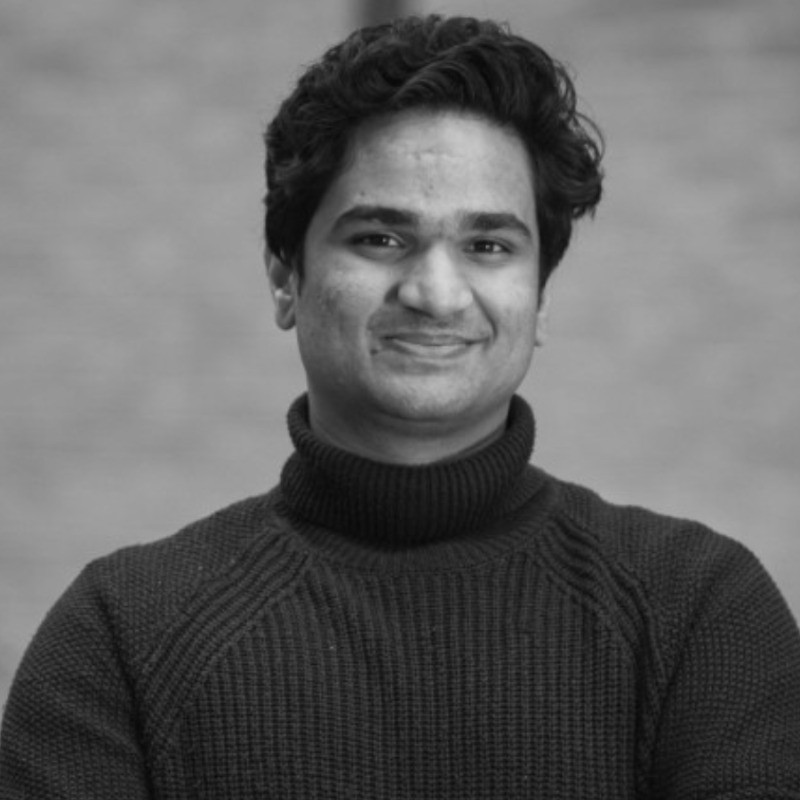
\includegraphics[width=2.0cm]{photo.jpg}
\end{minipage}
\vspace{-2pt}

% ================= SUMMARY =================
% -------- TAILOR: SUMMARY --------
\section{Summary}
I manage AI and automation projects from strategy through adoption. At FlowSpace I coordinated the rollout of AI-powered tools across the platform: I gathered requirements from workspace providers, planned deployment timelines, trained teams on new systems, and tracked adoption metrics. I bridged communication between technical and non-technical stakeholders, translating business needs into actionable specs for the engineering team. I managed the deployment of CRM integrations (OfficeRnD, Nexudus), workflow automations (n8n), and an AI listing pipeline that produced 900+ reviewed records. I oversaw the platform migration off a legacy stack, coordinating the cutover while keeping the product live for 4,500+ users. Based in Italy, EU long-term residence permit, available immediately.

% ================= SKILLS =================
% -------- TAILOR: SKILLS --------
\section{Skills}
\begin{itemize}
 \item \textbf{Project management:} Requirements gathering, stakeholder management, deployment planning, adoption tracking, training delivery, cross-functional coordination, Airtable, Asana
 \item \textbf{AI \& digital transformation:} Claude API, OpenAI API, AI agent deployment, LLM integration, prompt engineering, structured outputs, AI adoption strategy
 \item \textbf{Automation:} n8n, Make (Integromat), Zapier, Tray.ai, Microsoft Power Automate, workflow orchestration, process optimization, API integrations, OAuth2, webhooks
 \item \textbf{Technical:} Next.js, React, TypeScript, Node.js, PostgreSQL, Supabase, PHP, Laravel, dashboards, analytics, data transformations
\end{itemize}

% ================= EXPERIENCE =================
\section{Experience}

\role{\href{https://flowspace.co}{FlowSpace.co}}{Mar 2024 -- Aug 2026}{Full-Stack \& AI Engineer (Full-time, Freelance)}{London, UK (remote)}
\begin{itemize}
 \item Integrated OfficeRnD and Nexudus APIs end to end: connect flow, location sync, resource mapping, and automated bookings. Owned the full integration lifecycle from technical scoping to production.
 \item Ran technical onboarding for new workspace providers joining the platform. Configured their accounts, mapped their data, and resolved issues directly.
 \item Built an AI listing bot: takes a brochure in any format (PDF, web, photo, spreadsheet), drafts the listing via LLM, routes through human review, then pushes to the backend.
 \item Migrated the platform off a legacy stack to Next.js and Laravel. Mapped the data model, drove the cutover while the product stayed live. Scaled from 2,000 to 4,500+ users.
 \item Built CRM and GTM automations with n8n, plus AI support agents that answer queries against live platform data.
\end{itemize}

\role{\href{https://get2germany.com}{Get2Germany.com}}{Jan 2024 -- May 2024}{Developer \& Automation Specialist (Part-time)}{Berlin, Germany}
Integrated Google APIs, built AI tools to find courses, internships and jobs, and optimized the database. Stack: n8n, Google APIs.\\[1pt]

\role{\href{https://clubee.com}{Clubee.com}}{Sep 2023 -- Aug 2024}{Developer \& QA (Full-time, Freelance)}{Foetz, Luxembourg}
Integrated the Clubee API across the frontend, ran unit testing and QA, and built shop and federation-dashboard tools.\\[1pt]

\role{\href{https://tractionboard.co}{Tractionboard.co}}{Aug 2023 -- Oct 2023}{Developer (Internship)}{Utrecht, Netherlands}
Integrated ChatGPT/OpenAI and Sendgrid, built responsive designs, and debugged features.

% ================= FREELANCE PROJECTS =================
\section{Freelance Projects}
\begin{itemize}
 \item \textbf{\href{https://smarturlink.com/}{Urlink}} (2025), Project Manager \& AI-Assisted Developer. Built the platform with the client, gathering requirements and implementing automations. Stack: Next.js, Supabase, Netlify.
 \item \textbf{\href{https://ultrastrategy.com}{UltraStrategy}} (2024 to 2025), AI Automation Developer. Built a CV-parsing tool (LLM data extraction) with n8n and Eden AI.
 \item \textbf{\href{https://www.qomodo.me/}{Qomodo}} (2024 to 2025), AI Developer. Built a branch-management dashboard for companies.
\end{itemize}

% ================= CERTIFICATIONS =================
\section{Certifications}
Microsoft Copilot Studio Agent Academy \textbullet\ Microsoft: Introduction to building AI agents \textbullet\ Microsoft Power Automate \textbullet\ Tray.AI Build Practitioner (Sep 2024)

% ================= EDUCATION =================
\section{Education}
\textbf{Ca' Foscari University of Venice} \hfill Oct 2020 -- Jun 2024\\
BA Philosophy, International Studies \& Economics (Minor: Entrepreneurship)

\vspace{2pt}
{\small \textbf{Work authorization:} European Long Term Residence Permit (Italy), no sponsorship needed in the EU; available immediately. \quad \textbf{Languages:} Hindi (native), English (professional), Italian (beginner).}

\end{document}
